\chapter{Interpretation of the results}

\lettrine{T}{}his chapter is dedicated to the interpretation of the results of the \mph analysis presented in the previous chapter in terms of model independent limits and model dependent within the Minimal DM model. 

\section{Statistical model}
In particle physics one often searches for phenomena that have been predicted but not observed yet. Any analysis must be correlated by a quantitative evaluation of the significance of any signal collected. This is usually done by means of a \p or equivalently a Gaussian significance \emph{Z}~\cite{Cowan}.

Two kind of hypothesis can be defined. The null hypothesis $H_{0}$, which is the one to be tested against the alternative $H_{1}$. In a discovery analysis, in which new signal is looked for with no assumption on it, $H_{0}$ plays the role of background only hypothesis and $H_{1}$ is the signal plus backkground hypothesis. When setting limits on a particular model the roles are switched.

To summarize the outcome of an experiment and quantify the level of agreement between the data and an observed signal one can define a \p:
\begin{definizione}
  The \p of a distribution is the probability under the assumption of $H$ of finding data with equal or greater incompatibility with $H$.
\end{definizione}

An equivalent way to compute this kind of agreement is to turn the \p into Gaussian significance $Z$ by means of the inverse of the cumulative distribution of the standard Gaussian $\Phi^{-1}$ such that:
\begin{equation}
  Z = \Phi^{-1}(1-p)
\end{equation}

\section{The profile likelihood ratio}
The Likelihood function is defined as a function of a parameter of interest (POI) $\mu$, and a set of nuisance parameter $k_i$ and $\theta$~\cite{Cowan}.
A very common procedure to establish discovery (or exclusion) in particle physics is based on a likelihood ratio as a test statistic. Indeed, to test an hypothesized value of $\mu$ the \emph{profiled likelihood ratio} is used as the principal statistical estimator in this analysis, has been considered. It is defined as:
\begin{equation}
  \lambda(\mu) = \frac {\mathfrak{L}(\mu,\hat{\hat{\theta}})}{\mathfrak{L(\hat{\mu},\hat{\theta})}}
  \label{eqn:profiled}
\end{equation}
where in the numerator, $\hat{\hat{\theta}}$ is the conditional maximum-likelihood estimator (MLE) of $\theta$, or the value which maximizes $\mathfrak{L}$ for a given $\mu$ (therefore, it is a function of $\mu$), and the denominator is the maximized unconditional likelihood function.

\subsection{The $t_\mu$ test statistic}
The profiled likelihood ratio $\lambda(\mu)$ is by definition varied between 0 and 1 so that it is useful to define the corresponding $\tmu$ statistic as 
\begin{equation}
  t_{\mu} = -2 \log{\lambda(\mu)}
\end{equation}
which can be used to build a test statistic to quantify the discrepancy between data and the hypothesis where higher value of $t_{\mu}$ correspond to higher disagreement. The \p can also be evaluated, and its correspondance to $t_{\mu}$ is shown in \Fig{\ref{pvalue}}, as:
\begin{equation}
 p_{\mu}=\int_{t_{\mu,\textup{obs}}}^\infty f(t_\mu \vert \mu) dt_\mu
 \label{eqn:pdatmu}
\end{equation}

where $t_{\mu,\textup{obs}}$ is the value of $t_\mu$ observed from data and $f(t_\mu \vert \mu)$ is the probability density function of $t_\mu$ under the assumption of the POI value $\mu$. One can often assume that the presence of a new signal can only increase the mean event rate, which for a counting experiment can be evaluated as $E[n] = \mu s + b$ where $s$ corresponds to the signal events and $b$ is the background, so that we can consider parameter $\mu$ as positive so that an alternative test statistic $\tilde{t}_\mu$ can be defined. For a model in which $\mu>0$, if one finds that $\hat{\mu}<0$, the best level of agreement must be for $\mu=0$.

\begin{figure}[tp]
\centering
\subfloat[][]
{\includegraphics[width=.4\textwidth]{monophoton/pvaluea}}
\subfloat[][]
{\includegraphics[width=.416\textwidth]{monophoton/pvalueb}}
\caption{(\emph{a}) Relation between \p and $t_{\mu,\textup{obs}}$. (\emph{b}) Relation between the significance $Z$ and \p for a gaussian distribution $\varphi(x)$.}
\label{pvalue}
\end{figure}

\subsection{Test statistics for discovery and exclusion fit}
The presence of a signal can be quantified by testing the $\mu=0$ hypothesis against the $\mu>0$ one. Rejecting the $\mu=0$ hypothesis leads to the discovery of a new signal. On the other hand, without any observed excess of events in one or more SR(s), two methods set exclusion limits on new physics. These two fit strategies, complementary to the background only fit described in the previous chapter, are the discovery fit (model-independent) and the exclusion fit (model-dependent). Both fits are used to set upper limits on the POI, i.e. the number of events, by varying its value whithin a certain range and then interpolating for which POI value one finds \SI{95}{\percent} CL exclusion. For this reason, setting an upper limit is also called \emph{hypotest inversion}.

\subsubsection{The $q_0$ test for discovery of a positive signal}
In this scenario, rejecting the $\mu = 0$ hypothesis, i.e rejecting the background only hypothesis, leads to the discovery of a new signal.  An appropriate test statistic, the $q_0$, is therefore defined as follows:
\begin{equation}
q_0=
\left\{
\begin{aligned}
-2\log{\lambda(0)}\quad &\text{if}\quad \hat{\mu}\ge0\\
 0 \qquad&\text{if}\quad \hat{\mu}<0
\end{aligned}
\right.
\end{equation} 

Data shows lack of agreement with the background only hypothesis ($\hat{\mu}=0$), only if $q_0\ne0$. Using the observed value of $q_0$ one can quantify the level of disagreement between the data and the null hypothesis:
\begin{equation}
 p_{0}=\int_{q_{0,\textup{obs}}}^\infty f\left(q_0 \vert 0\right) dq_0
 \label{eqn:pdaq0}
\end{equation}

\subsubsection{The $q_\mu$ test for model dependent upper limits}
When searching for new phenomena if no excess is observed typically one would put constraints on potential new physiscs. Indeed, in a discovery fit the purpose is to set model-independent \SI{95}{\percent} CL upper limits on the number of Beyond Standard Model (BSM) events in SR. For no signal model in particular anyone can estimate the number of signal events predicted in a particular SR, in our case the already defined ``fiducial region'', and see wether a certain model has been excluded by current data or not.

This fit strategy is used with the purpose of studying a specific signal model. Exclusion limits can be performed for setting upper limit on the visible cross section of the model being tested. The model independent upper limit implements the signal only in the SR to set an upper limit on event one would observe, while the model dependent implements in in the SR and in every CR, in order to take into account any posssible signal contamination outside the SR. Note that this test is useful even in case of excess of events for which can be used to measure properties such as the signal strength.

For setting limits, a suitable test statistic is defined. However, now the null hypothesis is the signal plus background coexisting in the SR because a signal is supposed to be tested against the background only hypothesis. Therefore the $q_\mu$ test statistic is defined as:
\begin{equation}
q_\mu=
\left\{
\begin{aligned}
-2\log{\lambda(\mu)}\quad &\text{if}\quad \hat{\mu}\le\mu\\
 0 \qquad&\text{if}\quad \hat{\mu}>\mu
\end{aligned}
\right.
\end{equation} 
Once again the relation between $q_\mu$ and the \p is straighforward:
\begin{equation}
 p_{\mu}=\int_{q_{\mu,\textup{obs}}}^\infty f(q_\mu \vert \mu) dq_\mu
 \label{eqn:pdaqmu}
\end{equation}

In the context of exclusion limits, the $\cls$ statistic is mostly used replacing the \p. $\cls$ being derived from the \p is defined as:
\begin{equation}
	\cls=\frac{\text{p-value}(H_0)}{1-\text{p-value}(H_1)}
\end{equation}
which is the ratio between the \p given the signal and background and $1-$ the \p given the background only hypothesis.

Upper limits are then set for the value of $\mu$ whose corresponding $\cls$ is computed to be below the $0.05$ threshold.

\subsection{Experimental sensitivity}
\label{sec:sensitivity}
To characterize the sensitivity of an experiment, one normally reports the expected significance from a given measurement under different signal assumption.


In a model independent a discovery analysis one would like to know the median significance with which one would reject the background-only hypothesis under the assumption of a different ($\mu'$) signal strength. The median significance is obtained by replacing the ensamble of simulated data set with a single representative one, the so-called Asimov data set which it is easy to obtain the median values of $q_0$ and $q_\mu$.

The sensitivity of an experiment is illustrated in \Fig{\ref{fig:medianq}} which shows the PDF for $q_\mu$ when testing a signal strength $\mu$ and the distribution of $q_\mu$ when a signal strength $\mu'$ is being provided from the signal being tested.

The sensitivity of an experiment can be characterized by giving the \p corresponding to the median $q_\mu$, assuming an alternate value $\mu'$. 

When the distribution of the strength parameters $\mu'$ gets shifted to higher values, so does the median $q_\mu$. From \Eqn{\ref{eqn:pdaq0}} and \Eqn{\ref{eqn:pdaqmu}} it is clear that \p is pushed towards lower values. Now the hypotest inversion is finally revealed. What the fitting procedure achieved is to scan several values of $\mu$ and evaluate the median \p assuming $\mu'$. The computed upper limit is therefore the value of $\mu$ for which the \p gets under the threshold of \num{0.05}.

\begin{figure}[pt]
\centering
\includegraphics[width=0.5\textwidth]{interpretations/medianq}
\caption{Representation of the situation described in \Sect{\ref{sec:sensitivity}}. The observed distribution $f(q_\mu \vert \mu)$ is overlapped with the median $f(q_\mu \vert \mu')$ given by the asimptotic formul\ae~ according to which it has the form of an half chi squared distribution. The median $q_\mu$ is computed assuming the alternate value $\mu'$ and the result is used to calculate the \p for distribution $f(q_\mu \vert \mu)$.}
\label{fig:medianq}
\end{figure}

Note that all the $q_\mu$ distribution $f$ according to Wilks' theorem, can be approximated in the case of a large statistics as a one-degree of freedom (in case of one POI) $\chi^2$ distribution, regardless of the values taken by the nuisance parameters, see~\cite[\Sect{3}\!]{Cowan}. Alternatively one can obtain it by performing several pseudo-experiment, i.e. \emph{toys}, to get the right distribution even if they're always time expensive.

\section{Model-independent limit}
The model-independent fit purpose is to set upper limit on the number of BSM events that can be found in the SR. This can be achieved by counting the excess of events wrt SM prediction on the basis of a bogus signal model that is a single bin histogram with the bin value at 1. In this case the strength parameter $\mu$ assumes the meaning of number of events, and upper limits are given in terms of that. By rescaling with luminosity via \Eqn{\ref{eqn:Nevents}} one can obtain the corresponding upper limit on the visible cross section $\sigma_\textup{vis}=\sigma_\textit{th}\times A\times\epsilon$ where $\sigma_\textit{th}$ is the theorical cross section. The computed results for the fit are reported in \Tab{\ref{table.results.exclxsec.pval.upperlimit.SR}} and they exhibit good agreement with those published in~\cite{paperMP}. A cross section upper limit on new physics of \SI{5.91}{fb} has been established. Upper limit meaning is very simple: cross sections higher than the computed maximum are excluded, i.e. signal rate is strong and therefore as excess has to be observed. The CLs evlution versus the visible cross section being tested by the fit is reported in \Fig{\ref{fig:cls}}. The computed upper limit at \SI{95}{\percent} CL is the abscissa intersection between the observed/expected $\cls$ and the line $\cls=0.05$.


\begin{figure}[tp]
\centering
{\fontfamily{phv}\selectfont  
\small
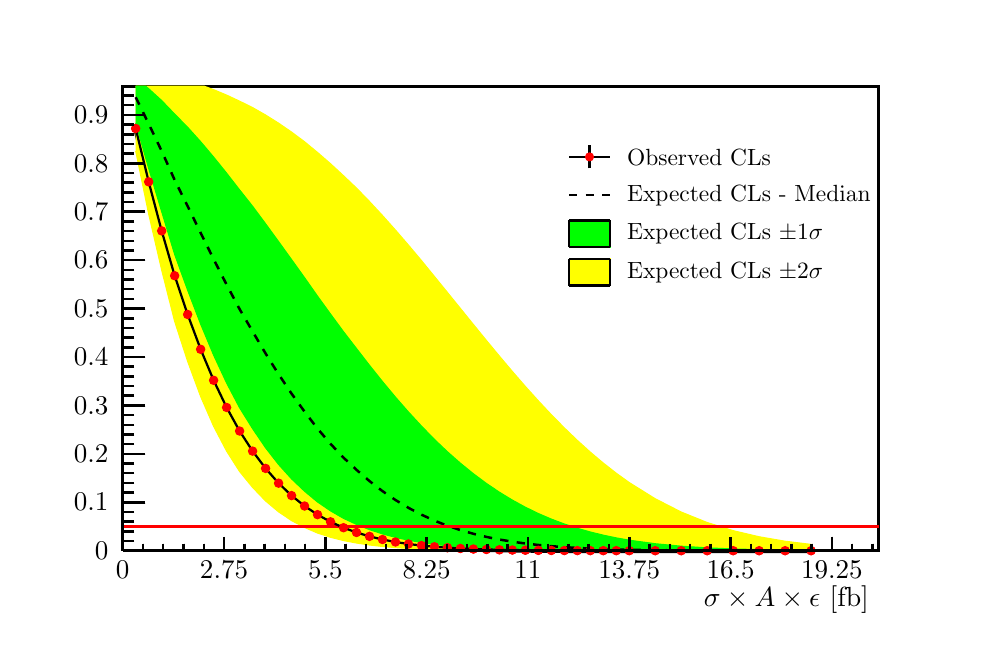
\begin{tikzpicture}[scale=0.6]
\pgfdeclareplotmark{cross} {
\pgfpathmoveto{\pgfpoint{-0.3\pgfplotmarksize}{\pgfplotmarksize}}
\pgfpathlineto{\pgfpoint{+0.3\pgfplotmarksize}{\pgfplotmarksize}}
\pgfpathlineto{\pgfpoint{+0.3\pgfplotmarksize}{0.3\pgfplotmarksize}}
\pgfpathlineto{\pgfpoint{+1\pgfplotmarksize}{0.3\pgfplotmarksize}}
\pgfpathlineto{\pgfpoint{+1\pgfplotmarksize}{-0.3\pgfplotmarksize}}
\pgfpathlineto{\pgfpoint{+0.3\pgfplotmarksize}{-0.3\pgfplotmarksize}}
\pgfpathlineto{\pgfpoint{+0.3\pgfplotmarksize}{-1.\pgfplotmarksize}}
\pgfpathlineto{\pgfpoint{-0.3\pgfplotmarksize}{-1.\pgfplotmarksize}}
\pgfpathlineto{\pgfpoint{-0.3\pgfplotmarksize}{-0.3\pgfplotmarksize}}
\pgfpathlineto{\pgfpoint{-1.\pgfplotmarksize}{-0.3\pgfplotmarksize}}
\pgfpathlineto{\pgfpoint{-1.\pgfplotmarksize}{0.3\pgfplotmarksize}}
\pgfpathlineto{\pgfpoint{-0.3\pgfplotmarksize}{0.3\pgfplotmarksize}}
\pgfpathclose
\pgfusepathqstroke
}
\pgfdeclareplotmark{cross*} {
\pgfpathmoveto{\pgfpoint{-0.3\pgfplotmarksize}{\pgfplotmarksize}}
\pgfpathlineto{\pgfpoint{+0.3\pgfplotmarksize}{\pgfplotmarksize}}
\pgfpathlineto{\pgfpoint{+0.3\pgfplotmarksize}{0.3\pgfplotmarksize}}
\pgfpathlineto{\pgfpoint{+1\pgfplotmarksize}{0.3\pgfplotmarksize}}
\pgfpathlineto{\pgfpoint{+1\pgfplotmarksize}{-0.3\pgfplotmarksize}}
\pgfpathlineto{\pgfpoint{+0.3\pgfplotmarksize}{-0.3\pgfplotmarksize}}
\pgfpathlineto{\pgfpoint{+0.3\pgfplotmarksize}{-1.\pgfplotmarksize}}
\pgfpathlineto{\pgfpoint{-0.3\pgfplotmarksize}{-1.\pgfplotmarksize}}
\pgfpathlineto{\pgfpoint{-0.3\pgfplotmarksize}{-0.3\pgfplotmarksize}}
\pgfpathlineto{\pgfpoint{-1.\pgfplotmarksize}{-0.3\pgfplotmarksize}}
\pgfpathlineto{\pgfpoint{-1.\pgfplotmarksize}{0.3\pgfplotmarksize}}
\pgfpathlineto{\pgfpoint{-0.3\pgfplotmarksize}{0.3\pgfplotmarksize}}
\pgfpathclose
\pgfusepathqfillstroke
}
\pgfdeclareplotmark{newstar} {
\pgfpathmoveto{\pgfqpoint{0pt}{\pgfplotmarksize}}
\pgfpathlineto{\pgfqpointpolar{44}{0.5\pgfplotmarksize}}
\pgfpathlineto{\pgfqpointpolar{18}{\pgfplotmarksize}}
\pgfpathlineto{\pgfqpointpolar{-20}{0.5\pgfplotmarksize}}
\pgfpathlineto{\pgfqpointpolar{-54}{\pgfplotmarksize}}
\pgfpathlineto{\pgfqpointpolar{-90}{0.5\pgfplotmarksize}}
\pgfpathlineto{\pgfqpointpolar{234}{\pgfplotmarksize}}
\pgfpathlineto{\pgfqpointpolar{198}{0.5\pgfplotmarksize}}
\pgfpathlineto{\pgfqpointpolar{162}{\pgfplotmarksize}}
\pgfpathlineto{\pgfqpointpolar{134}{0.5\pgfplotmarksize}}
\pgfpathclose
\pgfusepathqstroke
}
\pgfdeclareplotmark{newstar*} {
\pgfpathmoveto{\pgfqpoint{0pt}{\pgfplotmarksize}}
\pgfpathlineto{\pgfqpointpolar{44}{0.5\pgfplotmarksize}}
\pgfpathlineto{\pgfqpointpolar{18}{\pgfplotmarksize}}
\pgfpathlineto{\pgfqpointpolar{-20}{0.5\pgfplotmarksize}}
\pgfpathlineto{\pgfqpointpolar{-54}{\pgfplotmarksize}}
\pgfpathlineto{\pgfqpointpolar{-90}{0.5\pgfplotmarksize}}
\pgfpathlineto{\pgfqpointpolar{234}{\pgfplotmarksize}}
\pgfpathlineto{\pgfqpointpolar{198}{0.5\pgfplotmarksize}}
\pgfpathlineto{\pgfqpointpolar{162}{\pgfplotmarksize}}
\pgfpathlineto{\pgfqpointpolar{134}{0.5\pgfplotmarksize}}
\pgfpathclose
\pgfusepathqfillstroke
}
\definecolor{c}{rgb}{1,1,1};
\draw [color=c, fill=c] (0,0) rectangle (20,12.2874);
\draw [color=c, fill=c] (2,1.22874) rectangle (18,11.0587);
\definecolor{c}{rgb}{0,0,0};
\draw [c,line width=0.9] (2,1.22874) -- (2,11.0587) -- (18,11.0587) -- (18,1.22874) -- (2,1.22874);
\definecolor{c}{rgb}{1,1,1};
\draw [color=c, fill=c] (2,1.22874) rectangle (18,11.0587);
\definecolor{c}{rgb}{0,0,0};
\draw [c,line width=0.9] (2,1.22874) -- (2,11.0587) -- (18,11.0587) -- (18,1.22874) -- (2,1.22874);
\definecolor{c}{rgb}{0,0,0.6};
\draw [c,line width=0.9] (2,1.22874) -- (2.16,1.22874) -- (2.16,1.22874) -- (2.32,1.22874) -- (2.32,1.22874) -- (2.48,1.22874) -- (2.48,1.22874) -- (2.64,1.22874) -- (2.64,1.22874) -- (2.8,1.22874) -- (2.8,1.22874) -- (2.96,1.22874) -- (2.96,1.22874)
 -- (3.12,1.22874) -- (3.12,1.22874) -- (3.28,1.22874) -- (3.28,1.22874) -- (3.44,1.22874) -- (3.44,1.22874) -- (3.6,1.22874) -- (3.6,1.22874) -- (3.76,1.22874) -- (3.76,1.22874) -- (3.92,1.22874) -- (3.92,1.22874) -- (4.08,1.22874) -- (4.08,1.22874)
 -- (4.24,1.22874) -- (4.24,1.22874) -- (4.4,1.22874) -- (4.4,1.22874) -- (4.56,1.22874) -- (4.56,1.22874) -- (4.72,1.22874) -- (4.72,1.22874) -- (4.88,1.22874) -- (4.88,1.22874) -- (5.04,1.22874) -- (5.04,1.22874) -- (5.2,1.22874) -- (5.2,1.22874)
 -- (5.36,1.22874) -- (5.36,1.22874) -- (5.52,1.22874) -- (5.52,1.22874) -- (5.68,1.22874) -- (5.68,1.22874) -- (5.84,1.22874) -- (5.84,1.22874) -- (6,1.22874) -- (6,1.22874) -- (6.16,1.22874) -- (6.16,1.22874) -- (6.32,1.22874) -- (6.32,1.22874) --
 (6.48,1.22874) -- (6.48,1.22874) -- (6.64,1.22874) -- (6.64,1.22874) -- (6.8,1.22874) -- (6.8,1.22874) -- (6.96,1.22874) -- (6.96,1.22874) -- (7.12,1.22874) -- (7.12,1.22874) -- (7.28,1.22874) -- (7.28,1.22874) -- (7.44,1.22874) -- (7.44,1.22874) --
 (7.6,1.22874) -- (7.6,1.22874) -- (7.76,1.22874) -- (7.76,1.22874) -- (7.92,1.22874) -- (7.92,1.22874) -- (8.08,1.22874) -- (8.08,1.22874) -- (8.24,1.22874) -- (8.24,1.22874) -- (8.4,1.22874) -- (8.4,1.22874) -- (8.56,1.22874) -- (8.56,1.22874) --
 (8.72,1.22874) -- (8.72,1.22874) -- (8.88,1.22874) -- (8.88,1.22874) -- (9.04,1.22874) -- (9.04,1.22874) -- (9.2,1.22874) -- (9.2,1.22874) -- (9.36,1.22874) -- (9.36,1.22874) -- (9.52,1.22874) -- (9.52,1.22874) -- (9.68,1.22874) -- (9.68,1.22874) --
 (9.84,1.22874) -- (9.84,1.22874) -- (10,1.22874) -- (10,1.22874) -- (10.16,1.22874) -- (10.16,1.22874) -- (10.32,1.22874) -- (10.32,1.22874) -- (10.48,1.22874) -- (10.48,1.22874) -- (10.64,1.22874) -- (10.64,1.22874) -- (10.8,1.22874) --
 (10.8,1.22874) -- (10.96,1.22874) -- (10.96,1.22874) -- (11.12,1.22874) -- (11.12,1.22874) -- (11.28,1.22874) -- (11.28,1.22874) -- (11.44,1.22874) -- (11.44,1.22874) -- (11.6,1.22874) -- (11.6,1.22874) -- (11.76,1.22874) -- (11.76,1.22874) --
 (11.92,1.22874) -- (11.92,1.22874) -- (12.08,1.22874) -- (12.08,1.22874) -- (12.24,1.22874) -- (12.24,1.22874) -- (12.4,1.22874) -- (12.4,1.22874) -- (12.56,1.22874) -- (12.56,1.22874) -- (12.72,1.22874) -- (12.72,1.22874) -- (12.88,1.22874) --
 (12.88,1.22874) -- (13.04,1.22874) -- (13.04,1.22874) -- (13.2,1.22874) -- (13.2,1.22874) -- (13.36,1.22874) -- (13.36,1.22874) -- (13.52,1.22874) -- (13.52,1.22874) -- (13.68,1.22874) -- (13.68,1.22874) -- (13.84,1.22874) -- (13.84,1.22874) --
 (14,1.22874) -- (14,1.22874) -- (14.16,1.22874) -- (14.16,1.22874) -- (14.32,1.22874) -- (14.32,1.22874) -- (14.48,1.22874) -- (14.48,1.22874) -- (14.64,1.22874) -- (14.64,1.22874) -- (14.8,1.22874) -- (14.8,1.22874) -- (14.96,1.22874) --
 (14.96,1.22874) -- (15.12,1.22874) -- (15.12,1.22874) -- (15.28,1.22874) -- (15.28,1.22874) -- (15.44,1.22874) -- (15.44,1.22874) -- (15.6,1.22874) -- (15.6,1.22874) -- (15.76,1.22874) -- (15.76,1.22874) -- (15.92,1.22874) -- (15.92,1.22874) --
 (16.08,1.22874) -- (16.08,1.22874) -- (16.24,1.22874) -- (16.24,1.22874) -- (16.4,1.22874) -- (16.4,1.22874) -- (16.56,1.22874) -- (16.56,1.22874) -- (16.72,1.22874) -- (16.72,1.22874) -- (16.88,1.22874) -- (16.88,1.22874) -- (17.04,1.22874) --
 (17.04,1.22874) -- (17.2,1.22874) -- (17.2,1.22874) -- (17.36,1.22874) -- (17.36,1.22874) -- (17.52,1.22874) -- (17.52,1.22874) -- (17.68,1.22874) -- (17.68,1.22874) -- (17.84,1.22874) -- (17.84,1.22874) -- (18,1.22874);
\definecolor{c}{rgb}{0,0,0};
\draw [c,line width=0.9] (2,1.22874) -- (18,1.22874);
\draw [anchor= east] (18,0.2) node[color=c, rotate=0]{$\sigma\times A\times\epsilon$ [fb]};
\draw [c,line width=0.9] (2,1.52364) -- (2,1.22874);
\draw [c,line width=0.9] (2.42887,1.37619) -- (2.42887,1.22874);
\draw [c,line width=0.9] (2.85773,1.37619) -- (2.85773,1.22874);
\draw [c,line width=0.9] (3.2866,1.37619) -- (3.2866,1.22874);
\draw [c,line width=0.9] (3.71546,1.37619) -- (3.71546,1.22874);
\draw [c,line width=0.9] (4.14433,1.52364) -- (4.14433,1.22874);
\draw [c,line width=0.9] (4.5732,1.37619) -- (4.5732,1.22874);
\draw [c,line width=0.9] (5.00206,1.37619) -- (5.00206,1.22874);
\draw [c,line width=0.9] (5.43093,1.37619) -- (5.43093,1.22874);
\draw [c,line width=0.9] (5.85979,1.37619) -- (5.85979,1.22874);
\draw [c,line width=0.9] (6.28866,1.52364) -- (6.28866,1.22874);
\draw [c,line width=0.9] (6.71753,1.37619) -- (6.71753,1.22874);
\draw [c,line width=0.9] (7.14639,1.37619) -- (7.14639,1.22874);
\draw [c,line width=0.9] (7.57526,1.37619) -- (7.57526,1.22874);
\draw [c,line width=0.9] (8.00412,1.37619) -- (8.00412,1.22874);
\draw [c,line width=0.9] (8.43299,1.52364) -- (8.43299,1.22874);
\draw [c,line width=0.9] (8.86186,1.37619) -- (8.86186,1.22874);
\draw [c,line width=0.9] (9.29072,1.37619) -- (9.29072,1.22874);
\draw [c,line width=0.9] (9.71959,1.37619) -- (9.71959,1.22874);
\draw [c,line width=0.9] (10.1485,1.37619) -- (10.1485,1.22874);
\draw [c,line width=0.9] (10.5773,1.52364) -- (10.5773,1.22874);
\draw [c,line width=0.9] (11.0062,1.37619) -- (11.0062,1.22874);
\draw [c,line width=0.9] (11.4351,1.37619) -- (11.4351,1.22874);
\draw [c,line width=0.9] (11.8639,1.37619) -- (11.8639,1.22874);
\draw [c,line width=0.9] (12.2928,1.37619) -- (12.2928,1.22874);
\draw [c,line width=0.9] (12.7216,1.52364) -- (12.7216,1.22874);
\draw [c,line width=0.9] (13.1505,1.37619) -- (13.1505,1.22874);
\draw [c,line width=0.9] (13.5794,1.37619) -- (13.5794,1.22874);
\draw [c,line width=0.9] (14.0082,1.37619) -- (14.0082,1.22874);
\draw [c,line width=0.9] (14.4371,1.37619) -- (14.4371,1.22874);
\draw [c,line width=0.9] (14.866,1.52364) -- (14.866,1.22874);
\draw [c,line width=0.9] (15.2948,1.37619) -- (15.2948,1.22874);
\draw [c,line width=0.9] (15.7237,1.37619) -- (15.7237,1.22874);
\draw [c,line width=0.9] (16.1526,1.37619) -- (16.1526,1.22874);
\draw [c,line width=0.9] (16.5814,1.37619) -- (16.5814,1.22874);
\draw [c,line width=0.9] (17.0103,1.52364) -- (17.0103,1.22874);
\draw [c,line width=0.9] (17.0103,1.52364) -- (17.0103,1.22874);
\draw [c,line width=0.9] (17.4392,1.37619) -- (17.4392,1.22874);
\draw [c,line width=0.9] (17.868,1.37619) -- (17.868,1.22874);
\draw [anchor=base] (2,0.65) node[scale=0.976966, color=c, rotate=0]{0};
\draw [anchor=base] (4.14433,0.65) node[scale=0.976966, color=c, rotate=0]{2.75};
\draw [anchor=base] (6.28866,0.65) node[scale=0.976966, color=c, rotate=0]{5.5};
\draw [anchor=base] (8.43299,0.65) node[scale=0.976966, color=c, rotate=0]{8.25};
\draw [anchor=base] (10.5773,0.65) node[scale=0.976966, color=c, rotate=0]{11};
\draw [anchor=base] (12.7216,0.65) node[scale=0.976966, color=c, rotate=0]{13.75};
\draw [anchor=base] (14.866,0.65) node[scale=0.976966, color=c, rotate=0]{16.5};
\draw [anchor=base] (17.0103,0.65) node[scale=0.976966, color=c, rotate=0]{19.25};
\draw [c,line width=0.9] (2,1.22874) -- (2,11.0587);
\draw [anchor= east] (0.8,11.0587) node[scale=1, color=c, rotate=90]{$\cls$};
\draw [c,line width=0.9] (2.48,1.22874) -- (2,1.22874);
\draw [c,line width=0.9] (2.24,1.43372) -- (2,1.43372);
\draw [c,line width=0.9] (2.24,1.6387) -- (2,1.6387);
\draw [c,line width=0.9] (2.24,1.84369) -- (2,1.84369);
\draw [c,line width=0.9] (2.24,2.04867) -- (2,2.04867);
\draw [c,line width=0.9] (2.48,2.25365) -- (2,2.25365);
\draw [c,line width=0.9] (2.24,2.45863) -- (2,2.45863);
\draw [c,line width=0.9] (2.24,2.66362) -- (2,2.66362);
\draw [c,line width=0.9] (2.24,2.8686) -- (2,2.8686);
\draw [c,line width=0.9] (2.24,3.07358) -- (2,3.07358);
\draw [c,line width=0.9] (2.48,3.27857) -- (2,3.27857);
\draw [c,line width=0.9] (2.24,3.48355) -- (2,3.48355);
\draw [c,line width=0.9] (2.24,3.68853) -- (2,3.68853);
\draw [c,line width=0.9] (2.24,3.89351) -- (2,3.89351);
\draw [c,line width=0.9] (2.24,4.0985) -- (2,4.0985);
\draw [c,line width=0.9] (2.48,4.30348) -- (2,4.30348);
\draw [c,line width=0.9] (2.24,4.50846) -- (2,4.50846);
\draw [c,line width=0.9] (2.24,4.71344) -- (2,4.71344);
\draw [c,line width=0.9] (2.24,4.91843) -- (2,4.91843);
\draw [c,line width=0.9] (2.24,5.12341) -- (2,5.12341);
\draw [c,line width=0.9] (2.48,5.32839) -- (2,5.32839);
\draw [c,line width=0.9] (2.24,5.53337) -- (2,5.53337);
\draw [c,line width=0.9] (2.24,5.73836) -- (2,5.73836);
\draw [c,line width=0.9] (2.24,5.94334) -- (2,5.94334);
\draw [c,line width=0.9] (2.24,6.14832) -- (2,6.14832);
\draw [c,line width=0.9] (2.48,6.35331) -- (2,6.35331);
\draw [c,line width=0.9] (2.24,6.55829) -- (2,6.55829);
\draw [c,line width=0.9] (2.24,6.76327) -- (2,6.76327);
\draw [c,line width=0.9] (2.24,6.96825) -- (2,6.96825);
\draw [c,line width=0.9] (2.24,7.17324) -- (2,7.17324);
\draw [c,line width=0.9] (2.48,7.37822) -- (2,7.37822);
\draw [c,line width=0.9] (2.24,7.5832) -- (2,7.5832);
\draw [c,line width=0.9] (2.24,7.78818) -- (2,7.78818);
\draw [c,line width=0.9] (2.24,7.99317) -- (2,7.99317);
\draw [c,line width=0.9] (2.24,8.19815) -- (2,8.19815);
\draw [c,line width=0.9] (2.48,8.40313) -- (2,8.40313);
\draw [c,line width=0.9] (2.24,8.60811) -- (2,8.60811);
\draw [c,line width=0.9] (2.24,8.8131) -- (2,8.8131);
\draw [c,line width=0.9] (2.24,9.01808) -- (2,9.01808);
\draw [c,line width=0.9] (2.24,9.22306) -- (2,9.22306);
\draw [c,line width=0.9] (2.48,9.42804) -- (2,9.42804);
\draw [c,line width=0.9] (2.24,9.63303) -- (2,9.63303);
\draw [c,line width=0.9] (2.24,9.83801) -- (2,9.83801);
\draw [c,line width=0.9] (2.24,10.043) -- (2,10.043);
\draw [c,line width=0.9] (2.24,10.248) -- (2,10.248);
\draw [c,line width=0.9] (2.48,10.453) -- (2,10.453);
\draw [c,line width=0.9] (2.48,10.453) -- (2,10.453);
\draw [c,line width=0.9] (2.24,10.6579) -- (2,10.6579);
\draw [c,line width=0.9] (2.24,10.8629) -- (2,10.8629);
\draw [anchor= east] (1.9,1.22874) node[scale=0.976966, color=c, rotate=0]{0};
\draw [anchor= east] (1.9,2.25365) node[scale=0.976966, color=c, rotate=0]{0.1};
\draw [anchor= east] (1.9,3.27857) node[scale=0.976966, color=c, rotate=0]{0.2};
\draw [anchor= east] (1.9,4.30348) node[scale=0.976966, color=c, rotate=0]{0.3};
\draw [anchor= east] (1.9,5.32839) node[scale=0.976966, color=c, rotate=0]{0.4};
\draw [anchor= east] (1.9,6.35331) node[scale=0.976966, color=c, rotate=0]{0.5};
\draw [anchor= east] (1.9,7.37822) node[scale=0.976966, color=c, rotate=0]{0.6};
\draw [anchor= east] (1.9,8.40313) node[scale=0.976966, color=c, rotate=0]{0.7};
\draw [anchor= east] (1.9,9.42804) node[scale=0.976966, color=c, rotate=0]{0.8};
\draw [anchor= east] (1.9,10.453) node[scale=0.976966, color=c, rotate=0]{0.9};
\draw [c,line width=1.8] (2.27491,10.165) -- (2.54983,9.03623) -- (2.82474,7.99815) -- (3.09966,7.04863) -- (3.37457,6.22836) -- (3.64948,5.49118) -- (3.9244,4.83519) -- (4.19931,4.26022) -- (4.47423,3.76134) -- (4.74914,3.33651) -- (5.02406,2.97033)
 -- (5.29897,2.65788) -- (5.57388,2.39473) -- (5.8488,2.17458) -- (6.12371,1.99146) -- (6.39863,1.83977) -- (6.67354,1.71522) -- (6.94845,1.61416) -- (7.22337,1.53179) -- (7.49828,1.46553) -- (7.7732,1.4126) -- (8.04811,1.37059) -- (8.32302,1.3375)
 -- (8.59794,1.31155) -- (8.87285,1.29143) -- (9.14777,1.27589) -- (9.42268,1.26398) -- (9.69759,1.25491) -- (9.97251,1.24805) -- (10.2474,1.2429) -- (10.5223,1.23906) -- (10.7973,1.23621) -- (11.0722,1.23411) -- (11.3471,1.23258) -- (11.622,1.23147)
 -- (11.8969,1.23067) -- (12.1718,1.23009) -- (12.4467,1.22874) -- (12.7216,1.22874) -- (13.2715,1.22874) -- (13.8213,1.22874) -- (14.3711,1.22874) -- (14.921,1.22874) -- (15.4708,1.22874) -- (16.0206,1.22874) -- (16.5704,1.22874);
\definecolor{c}{rgb}{1,0,0};
\foreach \P in {(2.27491,10.165), (2.54983,9.03623), (2.82474,7.99815), (3.09966,7.04863), (3.37457,6.22836), (3.64948,5.49118), (3.9244,4.83519), (4.19931,4.26022), (4.47423,3.76134), (4.74914,3.33651), (5.02406,2.97033), (5.29897,2.65788),
 (5.57388,2.39473), (5.8488,2.17458), (6.12371,1.99146), (6.39863,1.83977), (6.67354,1.71522), (6.94845,1.61416), (7.22337,1.53179), (7.49828,1.46553), (7.7732,1.4126), (8.04811,1.37059), (8.32302,1.3375), (8.59794,1.31155), (8.87285,1.29143),
 (9.14777,1.27589), (9.42268,1.26398), (9.69759,1.25491), (9.97251,1.24805), (10.2474,1.2429), (10.5223,1.23906), (10.7973,1.23621), (11.0722,1.23411), (11.3471,1.23258), (11.622,1.23147), (11.8969,1.23067), (12.1718,1.23009), (12.4467,1.22968),
 (12.7216,1.22939), (13.2715,1.22905), (13.8213,1.22888), (14.3711,1.2288), (14.921,1.22877), (15.4708,1.22875), (16.0206,1.22874), (16.5704,1.22874)}{\draw[mark options={color=c,fill=c},mark size=2.402402pt,mark=*] plot coordinates {\P};}
\definecolor{c}{rgb}{1,1,0};
\draw [c, fill=c] (2.27491,11.0587) -- (3.72805,11.0587) -- (3.9244,10.9862) -- (4.19931,10.8715) -- (4.47423,10.7429) -- (4.74914,10.6069) -- (5.02406,10.4501) -- (5.29897,10.2775) -- (5.57388,10.0889) -- (5.8488,9.88384) -- (6.12371,9.65678) --
 (6.39863,9.41864) -- (6.67354,9.16464) -- (6.94845,8.90257) -- (7.22337,8.61933) -- (7.49828,8.32287) -- (7.7732,8.01457) -- (8.04811,7.69609) -- (8.32302,7.36913) -- (8.59794,7.03225) -- (8.87285,6.6945) -- (9.14777,6.35524) -- (9.42268,6.01592) --
 (9.69759,5.67883) -- (9.97251,5.34702) -- (10.2474,5.02182) -- (10.5223,4.7051) -- (10.7973,4.39965) -- (11.0722,4.10664) -- (11.3471,3.82737) -- (11.622,3.56322) -- (11.8969,3.31484) -- (12.1718,3.08307) -- (12.4467,2.8682) -- (12.7216,2.67025) --
 (13.2715,2.32762) -- (13.8213,2.04642) -- (14.3711,1.8245) -- (14.921,1.65254) -- (15.4708,1.52343) -- (16.0206,1.42882) -- (16.5704,1.36182) -- (16.5704,1.22874) -- (16.0206,1.22874) -- (15.4708,1.22874) -- (14.921,1.22874) -- (14.3711,1.22874) --
 (13.8213,1.22875) -- (13.2715,1.22877) -- (12.7216,1.22882) -- (12.4467,1.22886) -- (12.1718,1.22893) -- (11.8969,1.22902) -- (11.622,1.22917) -- (11.3471,1.22938) -- (11.0722,1.22969) -- (10.7973,1.23015) -- (10.5223,1.2308) -- (10.2474,1.23175) --
 (9.97251,1.2331) -- (9.69759,1.235) -- (9.42268,1.23768) -- (9.14777,1.24141) -- (8.87285,1.24657) -- (8.59794,1.25368) -- (8.32302,1.26349) -- (8.04811,1.27668) -- (7.7732,1.29441) -- (7.49828,1.31809) -- (7.22337,1.34949) -- (6.94845,1.3908) --
 (6.67354,1.44319) -- (6.39863,1.51274) -- (6.12371,1.60233) -- (5.8488,1.72003) -- (5.57388,1.86631) -- (5.29897,2.05066) -- (5.02406,2.28135) -- (4.74914,2.56788) -- (4.47423,2.90481) -- (4.19931,3.33623) -- (3.9244,3.86139) -- (3.64948,4.49267) --
 (3.37457,5.23582) -- (3.09966,6.08154) -- (2.82474,7.16878) -- (2.54983,8.35347) -- (2.27491,9.68871);
\definecolor{c}{rgb}{0,1,0};
\draw [c, fill=c] (2.27491,11.0587) -- (2.48616,11.0587) -- (2.54983,11.0059) -- (2.82474,10.7561) -- (3.09966,10.4694) -- (3.37457,10.1904) -- (3.64948,9.88508) -- (3.9244,9.55958) -- (4.19931,9.21854) -- (4.47423,8.86509) -- (4.74914,8.51832) --
 (5.02406,8.14786) -- (5.29897,7.77086) -- (5.57388,7.38975) -- (5.8488,7.00689) -- (6.12371,6.61545) -- (6.39863,6.23653) -- (6.67354,5.86321) -- (6.94845,5.50716) -- (7.22337,5.1515) -- (7.49828,4.8079) -- (7.7732,4.47815) -- (8.04811,4.16383) --
 (8.32302,3.86615) -- (8.59794,3.58336) -- (8.87285,3.322) -- (9.14777,3.07992) -- (9.42268,2.85667) -- (9.69759,2.65222) -- (9.97251,2.46671) -- (10.2474,2.29913) -- (10.5223,2.14873) -- (10.7973,2.01507) -- (11.0722,1.89692) -- (11.3471,1.79316) --
 (11.622,1.70274) -- (11.8969,1.62441) -- (12.1718,1.55707) -- (12.4467,1.49957) -- (12.7216,1.45076) -- (13.2715,1.37581) -- (13.8213,1.32356) -- (14.3711,1.28854) -- (14.921,1.26549) -- (15.4708,1.25079) -- (16.0206,1.24164) -- (16.5704,1.23613) --
 (16.5704,1.22874) -- (16.0206,1.22875) -- (15.4708,1.22877) -- (14.921,1.22881) -- (14.3711,1.22889) -- (13.8213,1.22906) -- (13.2715,1.22941) -- (12.7216,1.23012) -- (12.4467,1.2307) -- (12.1718,1.23151) -- (11.8969,1.23262) -- (11.622,1.23415) --
 (11.3471,1.23623) -- (11.0722,1.23904) -- (10.7973,1.2428) -- (10.5223,1.24782) -- (10.2474,1.25447) -- (9.97251,1.26319) -- (9.69759,1.27456) -- (9.42268,1.2893) -- (9.14777,1.30824) -- (8.87285,1.3324) -- (8.59794,1.36308) -- (8.32302,1.40214) --
 (8.04811,1.45051) -- (7.7732,1.51051) -- (7.49828,1.58446) -- (7.22337,1.67493) -- (6.94845,1.78484) -- (6.67354,1.91364) -- (6.39863,2.0717) -- (6.12371,2.25975) -- (5.8488,2.48778) -- (5.57388,2.74943) -- (5.29897,3.05426) -- (5.02406,3.40695) --
 (4.74914,3.81211) -- (4.47423,4.25368) -- (4.19931,4.77765) -- (3.9244,5.36794) -- (3.64948,6.025) -- (3.37457,6.74215) -- (3.09966,7.50068) -- (2.82474,8.40562) -- (2.54983,9.32091) -- (2.27491,10.2823);

%EXPECTED
\definecolor{c}{rgb}{0,0,0};
\draw [c,dashed,line width=0.9] (2.27491,10.8272) -- (2.54983,10.2634) -- (2.82474,9.68751) -- (3.09966,9.07404) -- (3.37457,8.51996) -- (3.64948,7.95632) -- (3.9244,7.39931) -- (4.19931,6.85891) -- (4.47423,6.34059) -- (4.74914,5.86928) --
 (5.02406,5.40265) -- (5.29897,4.96346) -- (5.57388,4.55295) -- (5.8488,4.17174) -- (6.12371,3.8119) -- (6.39863,3.4904) -- (6.67354,3.19784) -- (6.94845,2.9399) -- (7.22337,2.70178) -- (7.49828,2.48943) -- (7.7732,2.30135) -- (8.04811,2.13594) --
 (8.32302,1.99142) -- (8.59794,1.86484) -- (8.87285,1.757) -- (9.14777,1.66489) -- (9.42268,1.58657) -- (9.69759,1.52044) -- (9.97251,1.46514) -- (10.2474,1.41909) -- (10.5223,1.381) -- (10.7973,1.34982) -- (11.0722,1.32441) -- (11.3471,1.30386) --
 (11.622,1.28735) -- (11.8969,1.27418) -- (12.1718,1.26375) -- (12.4467,1.25554) -- (12.7216,1.24913) -- (13.2715,1.24037) -- (13.8213,1.23518) -- (14.3711,1.23223) -- (14.921,1.23058) -- (15.4708,1.22874) -- (16.0206,1.22874) -- (16.5704,1.22874);

%LINEA ORIZZONTALE PER  95 %CL
\definecolor{c}{rgb}{1,0,0};
\draw [c,line width=0.8] (2,1.7412) -- (18,1.7412);

%OBSERVED
\definecolor{c}{rgb}{0,0,0};
\draw [c,line width=0.8] (2.27491,10.165) -- (2.54983,9.03623) -- (2.82474,7.99815) -- (3.09966,7.04863) -- (3.37457,6.22836) -- (3.64948,5.49118) -- (3.9244,4.83519) -- (4.19931,4.26022) -- (4.47423,3.76134) -- (4.74914,3.33651) -- (5.02406,2.97033)
 -- (5.29897,2.65788) -- (5.57388,2.39473) -- (5.8488,2.17458) -- (6.12371,1.99146) -- (6.39863,1.83977) -- (6.67354,1.71522) -- (6.94845,1.61416) -- (7.22337,1.53179) -- (7.49828,1.46553) -- (7.7732,1.4126) -- (8.04811,1.37059) -- (8.32302,1.3375)
 -- (8.59794,1.31155) -- (8.87285,1.29143) -- (9.14777,1.27589) -- (9.42268,1.26398) -- (9.69759,1.25491) -- (9.97251,1.24805) -- (10.2474,1.2429) -- (10.5223,1.23906) -- (10.7973,1.23621) -- (11.0722,1.23411) -- (11.3471,1.23258) -- (11.622,1.23147)
 -- (11.8969,1.23067) -- (12.1718,1.23009) -- (12.4467,1.22874) -- (12.7216,1.22874) -- (13.2715,1.22874) -- (13.8213,1.22874) -- (14.3711,1.22874) -- (14.921,1.22874) -- (15.4708,1.22874) -- (16.0206,1.22874) -- (16.5704,1.22874);
\definecolor{c}{rgb}{1,0,0};
\foreach \P in {(2.27491,10.165), (2.54983,9.03623), (2.82474,7.99815), (3.09966,7.04863), (3.37457,6.22836), (3.64948,5.49118), (3.9244,4.83519), (4.19931,4.26022), (4.47423,3.76134), (4.74914,3.33651), (5.02406,2.97033), (5.29897,2.65788),
 (5.57388,2.39473), (5.8488,2.17458), (6.12371,1.99146), (6.39863,1.83977), (6.67354,1.71522), (6.94845,1.61416), (7.22337,1.53179), (7.49828,1.46553), (7.7732,1.4126), (8.04811,1.37059), (8.32302,1.3375), (8.59794,1.31155), (8.87285,1.29143),
 (9.14777,1.27589), (9.42268,1.26398), (9.69759,1.25491), (9.97251,1.24805), (10.2474,1.2429), (10.5223,1.23906), (10.7973,1.23621), (11.0722,1.23411), (11.3471,1.23258), (11.622,1.23147), (11.8969,1.23067), (12.1718,1.23009), (12.4467,1.22968),
 (12.7216,1.22939), (13.2715,1.22905), (13.8213,1.22888), (14.3711,1.2288), (14.921,1.22877), (15.4708,1.22875), (16.0206,1.22874), (16.5704,1.22874)}{\draw[mark options={color=c,fill=c},mark size=2.5pt,mark=*] plot coordinates {\P};}
\definecolor{c}{rgb}{1,1,1};
\draw [color=c, fill=c] (11.261,6.71554) rectangle (16.217,9.97067);
\definecolor{c}{rgb}{0,0,0};
\draw [anchor= west] (12.5,9.56378) node[scale=0.846704, color=c, rotate=0]{Observed CLs};
\draw [c,line width=0.8] (11.4468,9.56378) -- (12.3141,9.56378);
\draw [c,line width=0.8] (11.8805,9.31965) -- (11.8805,9.80792);
\definecolor{c}{rgb}{1,0,0};
\foreach \P in {(11.8805,9.56378)}{\draw[mark options={color=c,fill=c},mark size=2.402402pt,mark=*] plot coordinates {\P};}
\definecolor{c}{rgb}{0,0,0};
\draw [anchor= west] (12.5,8.75) node[scale=0.846704, color=c, rotate=0]{Expected CLs - Median};
\draw [c,dashed,line width=0.8] (11.4468,8.75) -- (12.3141,8.75);
\draw [anchor= west] (12.5,7.93622) node[scale=0.846704, color=c, rotate=0]{Expected CLs $\pm 1 \sigma$};
\definecolor{c}{rgb}{0,1,0};
\draw [c, fill=c] (11.4468,7.65139) -- (12.3141,7.65139) -- (12.3141,8.22104) -- (11.4468,8.22104);
\definecolor{c}{rgb}{0,0,0};
\draw [c,line width=0.9] (11.4468,8.22104) -- (12.3141,8.22104);
\draw [c,line width=0.9] (11.4468,7.65139) -- (12.3141,7.65139);
\draw [c,line width=0.9] (12.3141,7.65139) -- (12.3141,8.22104);
\draw [c,line width=0.9] (11.4468,7.65139) -- (11.4468,8.22104);
\draw [anchor= west] (12.5,7.12243) node[scale=0.846704, color=c, rotate=0]{Expected CLs $\pm 2 \sigma$};
\definecolor{c}{rgb}{1,1,0};
\draw [c, fill=c] (11.4468,6.83761) -- (12.3141,6.83761) -- (12.3141,7.40726) -- (11.4468,7.40726);
\definecolor{c}{rgb}{0,0,0};
\draw [c,line width=0.9] (11.4468,7.40726) -- (12.3141,7.40726);
\draw [c,line width=0.9] (11.4468,6.83761) -- (12.3141,6.83761);
\draw [c,line width=0.9] (12.3141,6.83761) -- (12.3141,7.40726);
\draw [c,line width=0.9] (11.4468,6.83761) -- (11.4468,7.40726);
\draw [c,line width=0.9] (2,1.22874) -- (18,1.22874);
\draw [c,line width=0.9] (2,1.52364) -- (2,1.22874);
\draw [c,line width=0.9] (2.42887,1.37619) -- (2.42887,1.22874);
\draw [c,line width=0.9] (2.85773,1.37619) -- (2.85773,1.22874);
\draw [c,line width=0.9] (3.2866,1.37619) -- (3.2866,1.22874);
\draw [c,line width=0.9] (3.71546,1.37619) -- (3.71546,1.22874);
\draw [c,line width=0.9] (4.14433,1.52364) -- (4.14433,1.22874);
\draw [c,line width=0.9] (4.5732,1.37619) -- (4.5732,1.22874);
\draw [c,line width=0.9] (5.00206,1.37619) -- (5.00206,1.22874);
\draw [c,line width=0.9] (5.43093,1.37619) -- (5.43093,1.22874);
\draw [c,line width=0.9] (5.85979,1.37619) -- (5.85979,1.22874);
\draw [c,line width=0.9] (6.28866,1.52364) -- (6.28866,1.22874);
\draw [c,line width=0.9] (6.71753,1.37619) -- (6.71753,1.22874);
\draw [c,line width=0.9] (7.14639,1.37619) -- (7.14639,1.22874);
\draw [c,line width=0.9] (7.57526,1.37619) -- (7.57526,1.22874);
\draw [c,line width=0.9] (8.00412,1.37619) -- (8.00412,1.22874);
\draw [c,line width=0.9] (8.43299,1.52364) -- (8.43299,1.22874);
\draw [c,line width=0.9] (8.86186,1.37619) -- (8.86186,1.22874);
\draw [c,line width=0.9] (9.29072,1.37619) -- (9.29072,1.22874);
\draw [c,line width=0.9] (9.71959,1.37619) -- (9.71959,1.22874);
\draw [c,line width=0.9] (10.1485,1.37619) -- (10.1485,1.22874);
\draw [c,line width=0.9] (10.5773,1.52364) -- (10.5773,1.22874);
\draw [c,line width=0.9] (11.0062,1.37619) -- (11.0062,1.22874);
\draw [c,line width=0.9] (11.4351,1.37619) -- (11.4351,1.22874);
\draw [c,line width=0.9] (11.8639,1.37619) -- (11.8639,1.22874);
\draw [c,line width=0.9] (12.2928,1.37619) -- (12.2928,1.22874);
\draw [c,line width=0.9] (12.7216,1.52364) -- (12.7216,1.22874);
\draw [c,line width=0.9] (13.1505,1.37619) -- (13.1505,1.22874);
\draw [c,line width=0.9] (13.5794,1.37619) -- (13.5794,1.22874);
\draw [c,line width=0.9] (14.0082,1.37619) -- (14.0082,1.22874);
\draw [c,line width=0.9] (14.4371,1.37619) -- (14.4371,1.22874);
\draw [c,line width=0.9] (14.866,1.52364) -- (14.866,1.22874);
\draw [c,line width=0.9] (15.2948,1.37619) -- (15.2948,1.22874);
\draw [c,line width=0.9] (15.7237,1.37619) -- (15.7237,1.22874);
\draw [c,line width=0.9] (16.1526,1.37619) -- (16.1526,1.22874);
\draw [c,line width=0.9] (16.5814,1.37619) -- (16.5814,1.22874);
\draw [c,line width=0.9] (17.0103,1.52364) -- (17.0103,1.22874);
\draw [c,line width=0.9] (17.0103,1.52364) -- (17.0103,1.22874);
\draw [c,line width=0.9] (17.4392,1.37619) -- (17.4392,1.22874);
\draw [c,line width=0.9] (17.868,1.37619) -- (17.868,1.22874);
\draw [c,line width=0.9] (2,1.22874) -- (2,11.0587);
\draw [c,line width=0.9] (2.48,1.22874) -- (2,1.22874);
\draw [c,line width=0.9] (2.24,1.43372) -- (2,1.43372);
\draw [c,line width=0.9] (2.24,1.6387) -- (2,1.6387);
\draw [c,line width=0.9] (2.24,1.84369) -- (2,1.84369);
\draw [c,line width=0.9] (2.24,2.04867) -- (2,2.04867);
\draw [c,line width=0.9] (2.48,2.25365) -- (2,2.25365);
\draw [c,line width=0.9] (2.24,2.45863) -- (2,2.45863);
\draw [c,line width=0.9] (2.24,2.66362) -- (2,2.66362);
\draw [c,line width=0.9] (2.24,2.8686) -- (2,2.8686);
\draw [c,line width=0.9] (2.24,3.07358) -- (2,3.07358);
\draw [c,line width=0.9] (2.48,3.27857) -- (2,3.27857);
\draw [c,line width=0.9] (2.24,3.48355) -- (2,3.48355);
\draw [c,line width=0.9] (2.24,3.68853) -- (2,3.68853);
\draw [c,line width=0.9] (2.24,3.89351) -- (2,3.89351);
\draw [c,line width=0.9] (2.24,4.0985) -- (2,4.0985);
\draw [c,line width=0.9] (2.48,4.30348) -- (2,4.30348);
\draw [c,line width=0.9] (2.24,4.50846) -- (2,4.50846);
\draw [c,line width=0.9] (2.24,4.71344) -- (2,4.71344);
\draw [c,line width=0.9] (2.24,4.91843) -- (2,4.91843);
\draw [c,line width=0.9] (2.24,5.12341) -- (2,5.12341);
\draw [c,line width=0.9] (2.48,5.32839) -- (2,5.32839);
\draw [c,line width=0.9] (2.24,5.53337) -- (2,5.53337);
\draw [c,line width=0.9] (2.24,5.73836) -- (2,5.73836);
\draw [c,line width=0.9] (2.24,5.94334) -- (2,5.94334);
\draw [c,line width=0.9] (2.24,6.14832) -- (2,6.14832);
\draw [c,line width=0.9] (2.48,6.35331) -- (2,6.35331);
\draw [c,line width=0.9] (2.24,6.55829) -- (2,6.55829);
\draw [c,line width=0.9] (2.24,6.76327) -- (2,6.76327);
\draw [c,line width=0.9] (2.24,6.96825) -- (2,6.96825);
\draw [c,line width=0.9] (2.24,7.17324) -- (2,7.17324);
\draw [c,line width=0.9] (2.48,7.37822) -- (2,7.37822);
\draw [c,line width=0.9] (2.24,7.5832) -- (2,7.5832);
\draw [c,line width=0.9] (2.24,7.78818) -- (2,7.78818);
\draw [c,line width=0.9] (2.24,7.99317) -- (2,7.99317);
\draw [c,line width=0.9] (2.24,8.19815) -- (2,8.19815);
\draw [c,line width=0.9] (2.48,8.40313) -- (2,8.40313);
\draw [c,line width=0.9] (2.24,8.60811) -- (2,8.60811);
\draw [c,line width=0.9] (2.24,8.8131) -- (2,8.8131);
\draw [c,line width=0.9] (2.24,9.01808) -- (2,9.01808);
\draw [c,line width=0.9] (2.24,9.22306) -- (2,9.22306);
\draw [c,line width=0.9] (2.48,9.42804) -- (2,9.42804);
\draw [c,line width=0.9] (2.24,9.63303) -- (2,9.63303);
\draw [c,line width=0.9] (2.24,9.83801) -- (2,9.83801);
\draw [c,line width=0.9] (2.24,10.043) -- (2,10.043);
\draw [c,line width=0.9] (2.24,10.248) -- (2,10.248);
\draw [c,line width=0.9] (2.48,10.453) -- (2,10.453);
\draw [c,line width=0.9] (2.48,10.453) -- (2,10.453);
\draw [c,line width=0.9] (2.24,10.6579) -- (2,10.6579);
\draw [c,line width=0.9] (2.24,10.8629) -- (2,10.8629);


\end{tikzpicture}
}
\caption{Evolution of the \p of the signal hypothesis ($\cls$) versus the visible cross section \mbox{\sv$=\sigma\times A\times\epsilon$}. The observed $\cls$ is shown with red dot markers and the black dashed lines represent the $\cls$ median get with the Asimov dataset. $1\sigma$ and $2\sigma$ uncertainties on $\cls$ expected are also reported. The red line indicates the $\cls$ threshold of \num{0.05} where the hypotest inversion is performed. Cross section values for which the correspondig $\cls$ is found to be below the red line are excluded at 95\% CL. }
\label{fig:cls}
\end{figure}




\subsubsection{Projections at \SI{120}{\ifb} and \SI{3}{ab^{-1}} integrated luminosity}
 In order to foresee future data prediction, Asimov dataset for integrated luminosity at \SI{120}{\ifb} and \SI{3}{ab^{-1}} were generated. The first value refers to actual estimate of the luminosity that will be delivered to ATLAS during \RunTwo, while the second is the prediction of the luminosity delivered in the whole LHC activity period. At \SI{120}{\ifb} the expected upper limit cross section is computed to be \SI{2.69}{fb}, at \SI{95}{\percent} CL, while at \SI{3}{ab^{-1}} is \SI{108}{ab}, at \SI{95}{\percent} CL as shown in \Tab{\ref{table.results.exclxsec.pval.upperlimit.SR}}.



\begin{table}[pt]
\centering
%\setlength{\tabcolsep}{0.0pc}
\begin{tabular}{ccccc}
\noalign{\smallskip}\toprule\noalign{\smallskip}
L [\ifb]&$\left({\rm \sigma_{\rm vis}}\right)_{\rm obs}^{95}$~[fb] &$\left({\rm \sigma_{\rm vis}}\right)_{\rm exp}^{95}$~[fb] &  $N_{\rm obs}^{95}$  & $N_{\rm exp}^{95}$  \\
\noalign{\smallskip}\midrule\noalign{\smallskip}
%%
$36.4$&$5.91$ &${ 8.86 }^{ +3.31 }_{ -2.39 } $ &  $215.1$ & $ { 322.6 }^{ +120.5 }_{ -87.0 }$ \\
\noalign{\smallskip}\midrule[.2pt]\noalign{\smallskip}
$120$&$1.79$ &${ 2.69 }^{ +1.00 }_{ -0.73 } $ &  $215.1$ & $ { 322.4 }^{ +120.5 }_{ -87.0 }$ \\
\noalign{\smallskip}\noalign{\smallskip}
$3000$&$0.072$ &${ 0.108 }^{ +0.040 }_{ -0.029 } $ &  $215.2$ & $ { 322.8 }^{ +120.5 }_{ -87.0 }$ \\
 
 
\noalign{\smallskip}\bottomrule\noalign{\smallskip}
\end{tabular}
\caption[Breakdown of upper limits.]{
Left to right:  First column reports the integrated luminosity used, then \SI{95}{\percent} CL upper limits on the visible cross section observed
followed by the expected
reporting the $\pm 1\sigma$
excursions are given. The third column shows the \SI{95}{\percent} CL upper limit on on the number of observed
signal events while the last reports the \SI{95}{\percent} CL upper limit on the expected number with $\pm 1\sigma$
excursions on the expectation, of background events.
Expected limits are given the absence of new physics.
First row of the table reports the result already published in~\cite{paperMP}, and below the solid line
outlooks at high luminosity is given. In the latter case the observed limit must be understood as coming from the Asimov dataset.
\label{table.results.exclxsec.pval.upperlimit.SR}}
\end{table}
%

\subsection{Fiducial cross section}

\begin{table}[pt]
 \centering
 \begin{tabular}{ccccc} 
 \noalign{\smallskip}\toprule\noalign{\smallskip} 
 Mass [GeV]& Cross section [pb]& $A$& $\epsilon$& $\mathcal{E}$\\ 
 \noalign{\smallskip}\midrule\noalign{\smallskip} 
\num{1}& \num{3.053e-01}& \num{0.134}& \num{0.6918}& \num{0.0927}\\ \smallskip
\num{10}& \num{2.958e-01}& \num{0.333}& \num{0.7078}& \num{0.2357}\\  \smallskip
\num{20}& \num{2.835e-01}& \num{0.398}& \num{0.7462}& \num{0.297}\\ \smallskip
\num{30}& \num{2.516e-01}& \num{0.416}& \num{0.7791}& \num{0.3241}\\ \smallskip
\num{40}& \num{1.066e-01}& \num{0.425}& \num{0.7894}& \num{0.3355}\\ \smallskip
\num{50}& \num{1.571e-02}& \num{0.443}& \num{0.7619}& \num{0.3375}\\ \smallskip
\num{60}& \num{1.069e-02}& \num{0.452}& \num{0.7515}& \num{0.3397}\\ \smallskip
\num{70}& \num{8.300e-03}& \num{0.454}& \num{0.7762}& \num{0.3524}\\ \smallskip
\num{80}& \num{6.742e-03}& \num{0.465}& \num{0.7708}& \num{0.3584}\\\smallskip 
\num{90}& \num{5.554e-03}& \num{0.474}& \num{0.7730}& \num{0.3664}\\ \smallskip 
\num{100}& \num{4.659e-03}& \num{0.473}& \num{0.7738}& \num{0.3660}\\ \smallskip 
\num{200}& \num{1.164e-03}& \num{0.508}& \num{0.7516}& \num{0.3818}\\ \smallskip
\num{300}& \num{4.026e-04}& \num{0.507}& \num{0.7596}& \num{0.3851}\\ \smallskip 
\num{400}& \num{1.638e-04}& \num{0.528}& \num{0.7413}& \num{0.3914}\\ \smallskip
\num{500}& \num{7.428e-05}& \num{0.540}& \num{0.7369}& \num{0.3979}\\ \smallskip 
\num{600}& \num{3.642e-05}& \num{0.530}& \num{0.7454}& \num{0.3951}\\ \smallskip
\num{700}& \num{1.881e-05}& \num{0.539}& \num{0.7469}& \num{0.4026}\\ \smallskip
\num{800}& \num{1.009e-05}& \num{0.539}& \num{0.7419}& \num{0.3999}\\ \smallskip
\num{900}& \num{5.569e-06}& \num{0.532}& \num{0.7397}& \num{0.3935}\\ \smallskip
\num{1000}& \num{3.183e-06}& \num{0.535}& \num{0.7564}& \num{0.4047}\\ \smallskip
\num{1200}& \num{1.084e-06}& \num{0.539}& \num{0.7468}& \num{0.4025}\\ 
	\noalign{\smallskip}\bottomrule\noalign{\smallskip} 
 \end{tabular} 
 \caption{Mass samples considered with the corresponding cross section in pb are reported. For each of them fiducial acceptance, fiducial efficiency and total efficiency are also listed. In the analysis the fiducial acceptance was computed first, then the total efficiency and finally the fiducial efficiency was calculated by a mere ratio between them} 
 \label{tab:eff} 
 \end{table}
 

\begin{figure}[p]
\centering
\subfloat[][\label{subfig:exclMI}]
{\includegraphics[width=.75\textwidth]{interpretations/exclusionplot}} \\
\subfloat[][\label{subfig:exclMIZ}]
{\includegraphics[width=.75\textwidth]{interpretations/exclusionplotZoom}} \quad
\caption{Upper limit on $\chi_0$ mass rescaled on the computed total efficiency for every mass sample. Solid line represents the upper limit on the visible cross section rescaled by total efficiency $\left(A\times\epsilon\right)$. Dashed black line is the expected upper limit and finally the dashed red line shows the theorical cross section. ($b$) is the enlarged version of ($a$) in the crossing region. Masses below \SI{\sim 50}{\gev} are rejected by the analysis.}
\label{fig:exclMI}
\end{figure}

\begin{figure}[p]
\centering
\subfloat[][ \SI{120}{\ifb} upper limit \label{subfig:120mi}]
{\includegraphics[width=.45\textwidth]{interpretations/exclusionplot120}} \quad
\subfloat[][ \SI{120}{\ifb} upper limit, enlarged\label{subfig:120miZ}]
{\includegraphics[width=.45\textwidth]{interpretations/exclusionplotZoom120}} \\
\subfloat[][ \SI{3}{ab^{-1}} upper limit\label{subfig:3000mi}]
{\includegraphics[width=.45\textwidth]{interpretations/exclusionplot3000}} \quad
\subfloat[][\SI{3}{ab^{-1}} upper limit, enlarged\label{subfig:3000miZ}]
{\includegraphics[width=.45\textwidth]{interpretations/exclusionplotZoom3000}} \\
\caption{Upper limits projections at \SI{120}{\ifb} and \SI{3}{ab^{-1}} plot rescaled for the total efficiency computed for every mass sample. Dashed black line represents the expected and the dashed red line is the theorical cross section. Enlargements in the crossing range are also reported.}
\label{fig:outlookmi}
\end{figure}

In order to put constrain on model not covered in this analysis, a ``fiducial region'' was defined with kinematic cuts given in \Sect{\ref{sec:truth}}, corresponding to a signal region selection applied at the truth level. A fiducial cross section can be defined starting from the visible cross section divided by the reconstruction efficiency.

Total efficiency $\left(\text{Eff}_\textup{tot}\right)$ can be defined as the ratio between events passing the selections at reconstruction level in the SR $\left(N_\textup{reco}\right)$ and the total number of events generated $\left(N_\textup{total}\right)$, which for the signals being tested is \num{10000}. It can be decomposed into a fiducial acceptance $A$ and a fiducial reconstruction efficiency $\epsilon$:
\begin{equation}
	\text{Eff}_\textup{tot}=\frac{N_\textup{reco}}{N_\textup{total}}=A\times\epsilon
\end{equation}

Fiducial acceptance is defined as:
\begin{equation}
	A=\frac{N_\textup{fid}}{N_\textup{total}}
	\label{eqn:accfid}
\end{equation}
or the ratio between the number of events passing the truth-level fiducial cuts $\left(N_\textup{fid}\right)$ and the total numer of events generated, and the fiducial reconstruction efficiency is:
\begin{equation}
	\epsilon=\frac{N_\textup{reco}}{N_\textup{fid}}
	\label{eqn:efffid}
\end{equation}

Theoretical cross section, fiducial acceptance, fiducial efficiency and total efficiency for the \num{21} mass points considered are reported in \Tab{\ref{tab:eff}}. Lower acceptance values for small masses are due to the \met shape. As we can see from \Fig{\ref{fig:validation}} those masses have the peak in the \met distribution shifted to the left so that fewer events would pass the truth level selection. Fiducial efficiency ranges in \SIrange{69}{79}{\percent}.

Given the model independent upper limit on the vidible cross section from \Tab{\ref{table.results.exclxsec.pval.upperlimit.SR}}, for every mass point the corresponding $\left(\text{Eff}_\textup{tot}\right)$ can be used to rescale it and bring it back to the theoretical cross section since $\sigma_\textup{theo}^\textup{U.L.}=\sigma_\textup{vis}^\textup{U.L.}/\left(A\times\epsilon\right)$, where U.L. stands for the \sv upper limit. Note that even if the samples being tested are at truth level, the total efficiency $\epsilon$ computed from the full simulated events, see \Sect{\ref{sec:full}}, have been used.

These values have been compared to the theorical cross section reported in \Tab{\ref{tab:eff}}. The resulting plot, made from the truth level reconstruction, is pictured in \Fig{\ref{subfig:exclMI}}. Values of the theorical cross section above the observed line are excluded by the analysis.

An enlarged plot on the area of interest is also reported in  \Fig{\ref{subfig:exclMIZ}}. From the plots, \chizero masses below \SI{\sim50}{\GeV} are excluded.

The same procedure has been repeated for the high luminosity scenarios and the analysis is expected to exclude masses below \SI{\sim100}{\gev} for the \SI{120}{\ifb} case and \SI{\sim400}{\gev} at \SI{3}{ab^{-1}}. 

\section{Interpretation at full simulation level}
\label{sec:full}
Full simulated simulated and described in Chapter 3, were used to perform an exclusion (model-dependent) fit for the Minimal DM model to obtain upper limits on \chizero cross section production, on number of events yield, in the SR.

Now the POI is the signal strength $\mu=\sigma_\textup{{vis}}/\sigma_{\textup{theo}}$ and upper limits were set on it. In order to obtain the limit on the cross section, for each mass, the theorical cross section reported in \Tab{\ref{tab:eff}} was multiplied by the computed upper limit on the signal strength. 

The computed limit on the cross section of \chizero production can be expressed as:
\begin{equation}
	\sigma_{\chi_0}^\textup{U.L.}=\frac{\mu\times\sigma_\textup{vis}}{A\times\epsilon}=\mu\times\sigma_\textup{theo}
\end{equation}

Note that the dominant background \znng has a \SI{760}{fb} cross section and signal cross section varies in the range \SIrange{0.001}{305}{fb}, being \SI{\sim1}{fb} on average. On the other hand the SR was optimized so that the ratio of signal over background yields in the SR is \num{0.05} so that the SR selection enhances the probability of finding signal over background~\cite{mgiulia}.

Upper limit values for a mass $m_i$ below \num{1} indicates that this mass could be certainly excluded by the analysis. Indeed, the upper limit cross section would be $\sigma_\textup{vis}\times \mu^\textup{U.L.}$ and when $\mu^\textup{U.L.} \le 1$, the visible cross section results lower than the theorical and therefore rejected.

In \Tab{\ref{tab:mu}} the observed and expected upper limit, on the strength parameter $\mu$, are reported. The POI goes above $1$ between \SI{60}{\gev} and \SI{70}{\gev} so that mass excluded from the full simulated sample is \SI{\sim60}{\gev}. In \Fig{\ref{fig:exclMD}} the upper limit in terms of the theoretical cross section is shown. 

The truth level and full simulation approach are quite in agreement. The lack of perfect is given from the fact that for the latter, no systematic uncertainties have been taken into account.

\input{interpretations/tableMuSig}

\begin{figure}[tp]
\centering
\subfloat[][\label{subfig:exclMD}]
{\includegraphics[width=.75\textwidth]{interpretations/exclusionplotMD}} \\
\subfloat[][\label{subfig:exclMDZ}]
{\includegraphics[width=.75\textwidth]{interpretations/exclusionplotZoomMD}} \quad
\caption{Model dependent upper limit on $\chi_0$ mass rescaled on the computed total efficiency for data yield. Solid line represents the upper limit on the visible cross section rescaled by total efficiency $\left(A\times\epsilon\right)$. Dashed black line is the expected upper limit and finally the dashed red line shows the theorical cross section. ($b$) is the enlarged version of ($a$) in the critical region. Mass below \SI{\sim 60}{\gev} are rejected by the analysis.}
\label{fig:exclMI}
\end{figure}










